To study excited \cascade baryons the simulation of signal events is needed.
For this study 1.5 million signal events have been generated.
The decay channel for the simulation is shown in figure \ref{fig:eventgeneration_decaychannel}. 

\begin{figure}[htbp]
	\centering
			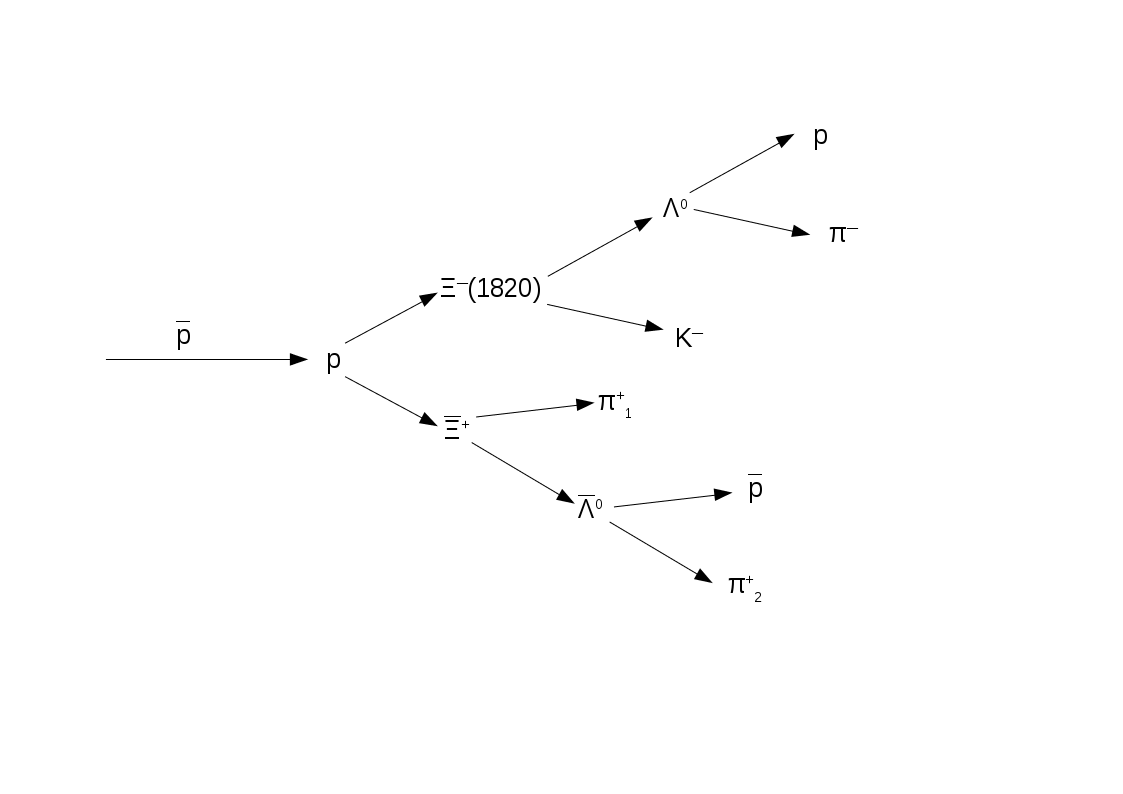
\includegraphics[width=1.00\textwidth]{./plots/DecayChannelXi1820.png}
	\caption{Simulated decay channel}
	\label{fig:eventgeneration_decaychannel}
\end{figure}

For the charge conjungated channel further 1.5 million events were generated.
The used parameters for the event generation are shown in table \ref{tab:eventgeneration_parameter}.

\begin{table}[tbp]
	\caption{Parameter for event generation}
	\label{tab:eventgeneration_parameter}
	\centering
	\begin{tabular}{ll}
		\hline
		Parameter & Value \\
		\hline
		\hline
		Beam momentum & 4.6 \massunit \\
		Production & PHSP \\
		Tracking & Ideal \\
		Particle ID & Ideal \\\hline
		 
	\end{tabular}
\end{table}

The chosen beam momentum of $p_{\bar{\mt{p}}} = 4.6\unit{GeV/c}$ is 100 MeV above the production threshold of \excitedcascade and \anticascade.
The production cross section is expected to be of the same order ($\sim \mu\mt{b}$) as for \cascade \cite{PANDAphysics2009}.\\
\vspace{11pt} 

The used software versions for Pandaroot and the external software package is listed in table \ref{tab:eventgeneration_software} 

\begin{table}[tb]
	\centering
	\caption{Used software versions}
	\label{tab:eventgeneration_software}
	\begin{tabular}{ll}
		\hline
		Software & Version \\
		\hline
		\hline
		FairSoft & mar15\\
		FairRoot & v-15.03a \\
		PandaRoot & trunk revision 28555 \\
		Geant & 3\\
		Genfit & 1\\\hline
			 
	\end{tabular}
\end{table}


Since now \excitedcascade was not defined in the evt.pdl file. 
The Lines in the code sniplet \ref{lst:eventgeneration_evtpdl} show how the particle is added to the file.
The properties of \excitedcascade comming from \cite{PDG} are written down in table \ref{tab:eventgeneration_Xivalues}.

\begin{lstlisting}[caption={sniplet from evt.pdl}\label{lst:eventgeneration_evtpdl}, captionpos=t,breaklines=true]
add  p Particle Xi(1820)- 23314 1.8230000e+00 2.4000000e-02 2.0000000e-01 -3 3 0.0000000e+00 23314
add  p Particle anti-Xi(1820)+ -23314 1.8230000e+00 2.4000000e-02 2.0000000e-01 3 3 0.0000000e+00 -23314
\end{lstlisting}

\begin{table}[htbp]
	\centering
	\caption{Properties of \excitedcascade and \excitedanticascade. The values are taken from \cite{PDG}}
	\label{tab:eventgeneration_Xivalues}
	\begin{tabular}{lllllll}
		\hline
		Particle & J & I & P & Charge & Mass  & Width \\
		\hline
		\hline
		\excitedcascade & $\frac{3}{2}$ & $\frac{1}{2}$ & ($-1$) & ($-1$) & ($1.823 \pm 5$)\massunit & ($0.024 \pm 6) $ GeV \\
		\excitedanticascade & $\frac{3}{2}$ & $\frac{1}{2}$ & ($-1$) & 1 & ($1.823 \pm 5$)\massunit & ($0.024 \pm 6) $ GeV\\
		\hline
		  
	\end{tabular}
\end{table}

The generated transverse momentum against the longitudinal momentum for \lam, \alam, \anticascade and \excitedcascade is 
presented in figure \ref{fig:MC_lambda0_pt_vs_pz}% -- \ref{fig:MC_xi_pt_vs_pz}.\\


\begin{figure}
	\subfigure[\lam]{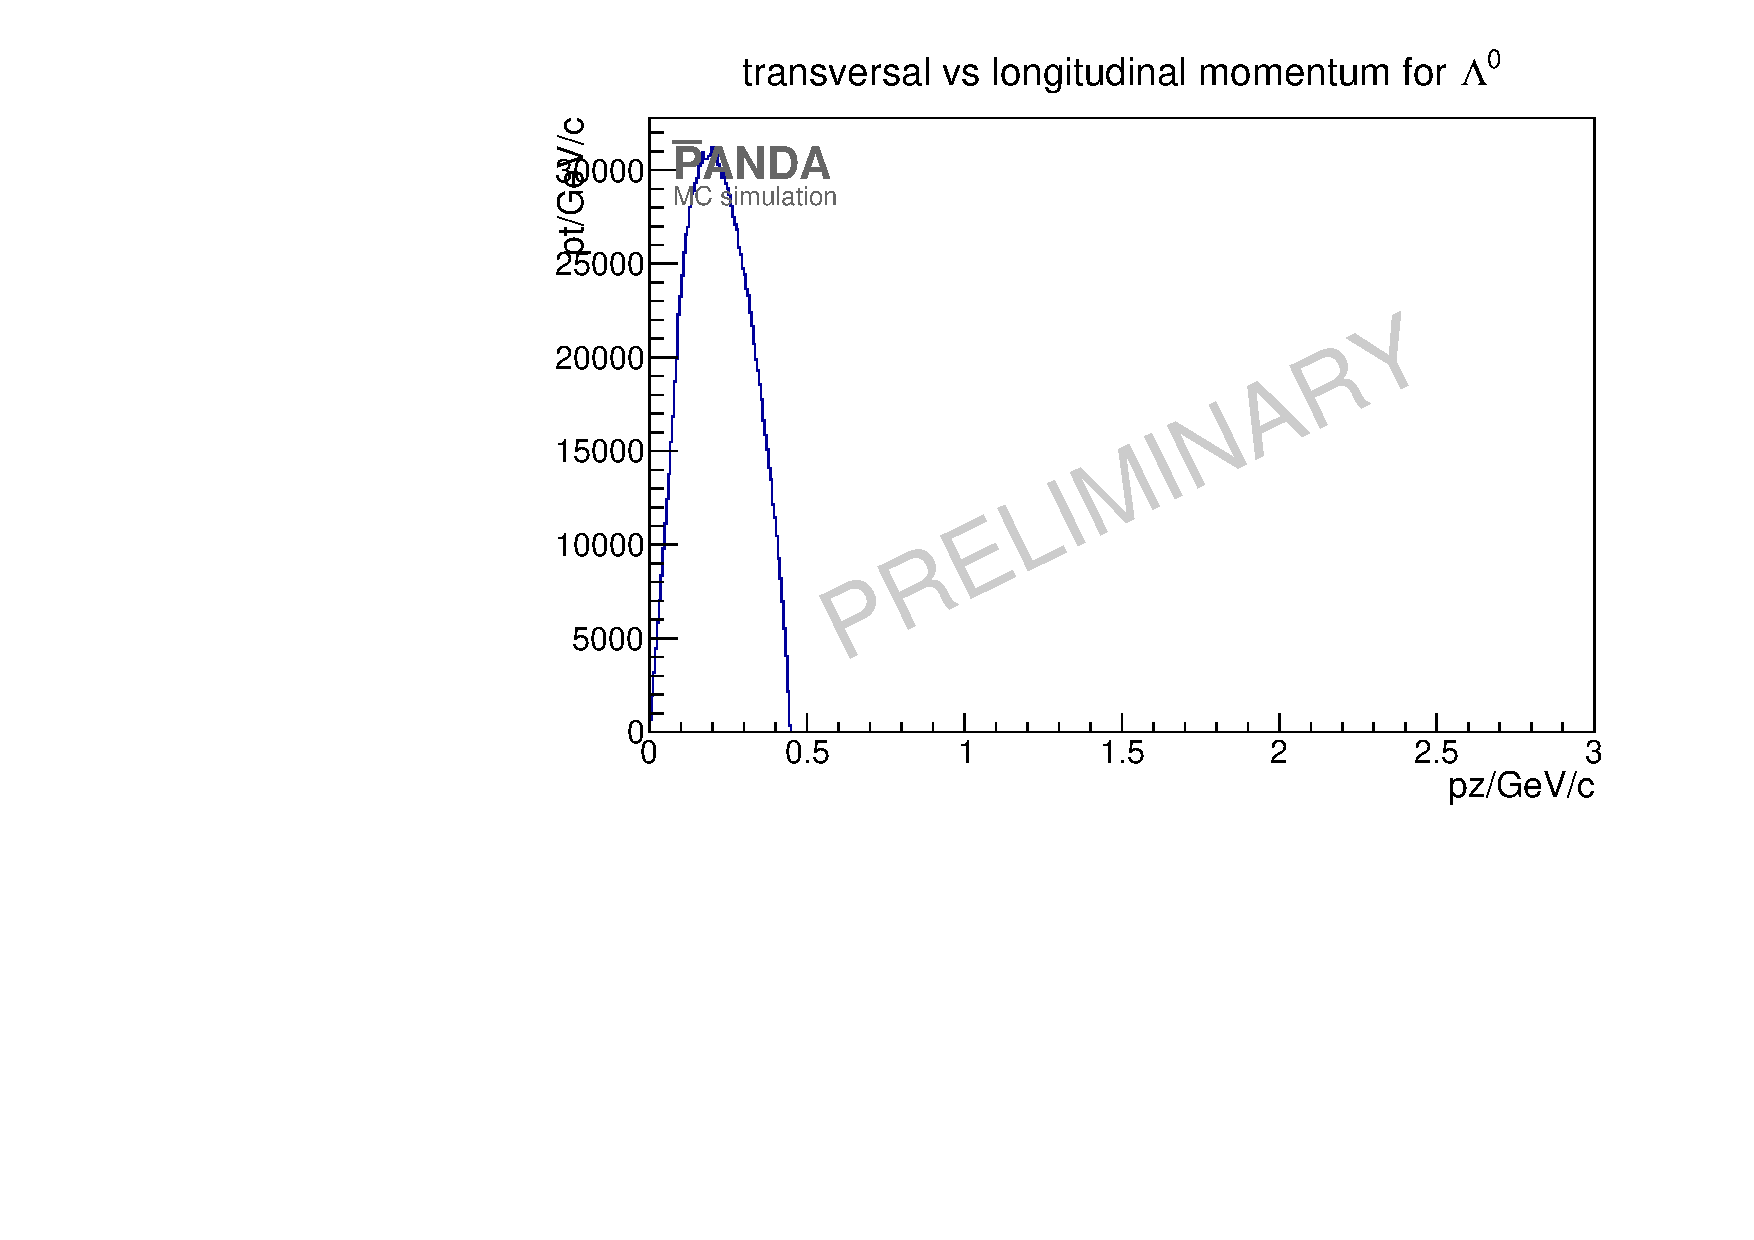
\includegraphics[width=0.49\textwidth]{./plots/lambda0/Lambda0_MC_pt_vs_pz.pdf}}
	\subfigure[\alam]{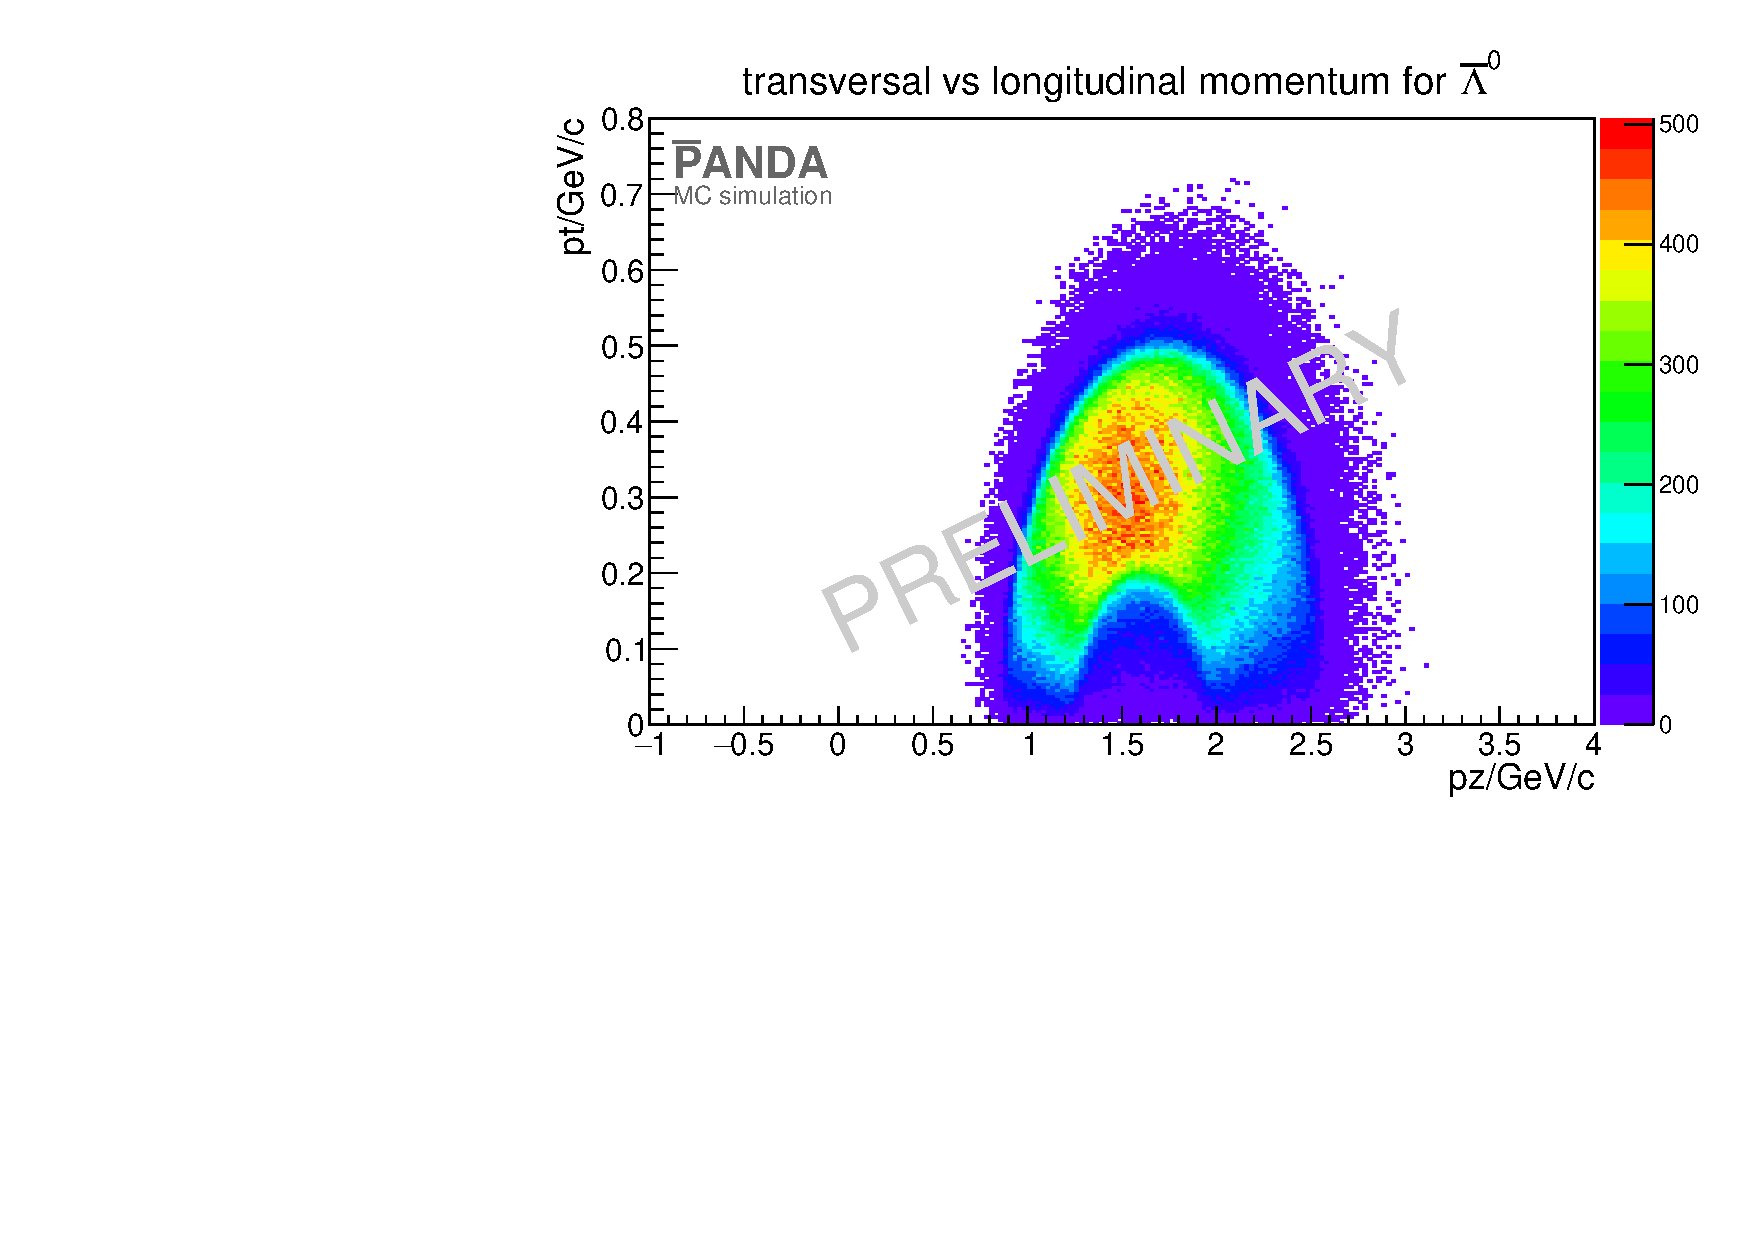
\includegraphics[width=0.49\textwidth]{./plots/antilambda0/AntiLambda0_MC_pt_vs_pz.pdf}}
	\caption{Figure a) shows the transverse momentum on the y axis against the longitudinal momentum on the x axis for \lam. Figure b) 
			shows the same distribution for \alam.}
	\label{fig:MC_lambda0_pt_vs_pz}
\end{figure}


\begin{figure}
	\subfigure[\anticascade]{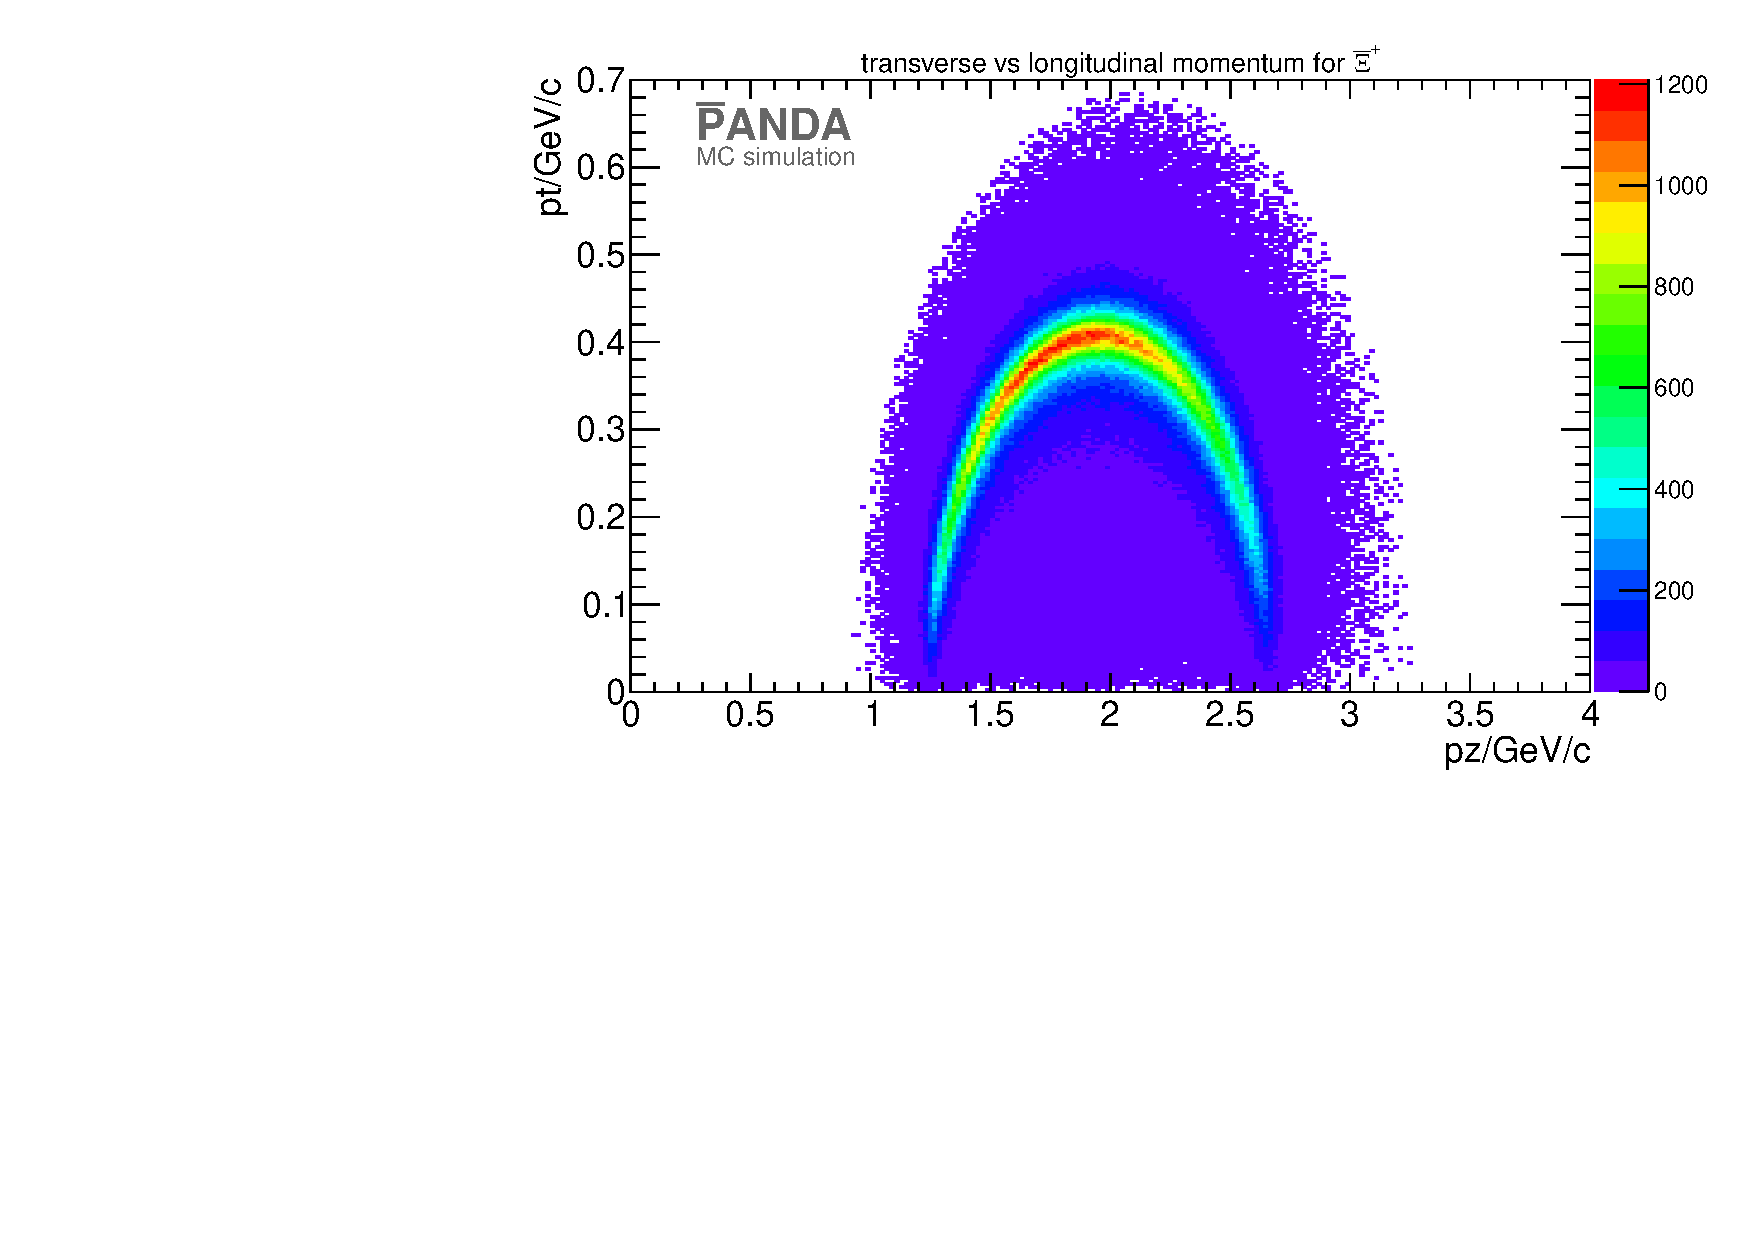
\includegraphics[width=0.49\textwidth]{./plots/Xi/XiPlus_MC_pt_vs_pz.pdf}}
	\subfigure[\excitedcascade]{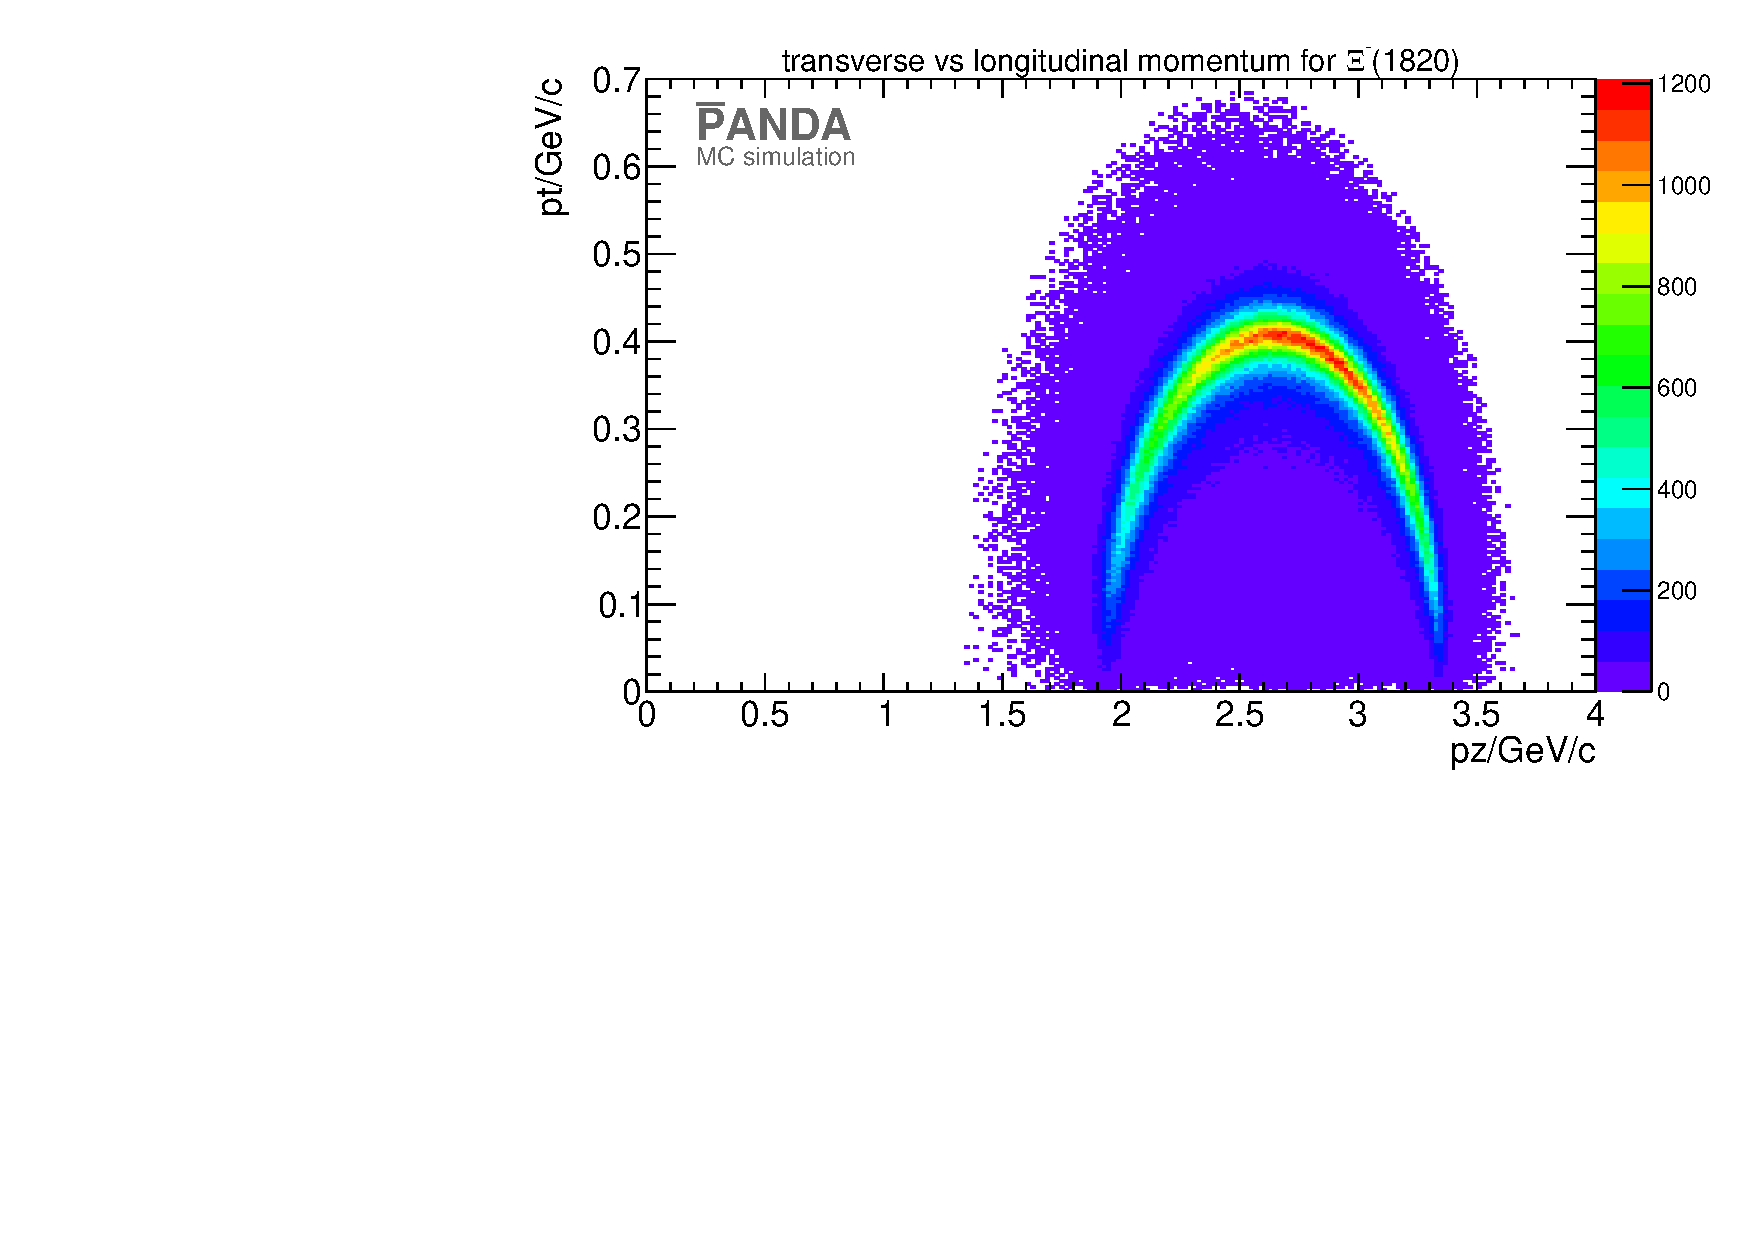
\includegraphics[width=0.49\textwidth]{./plots/Xi1820/XiMinus1820_MC_pt_vs_pz.pdf}}
	\caption{Figure a) shows transversal against the longitudinal momentum distribution for \anticascade. Figure b) 
			transversal versus longitudinal momentum distribution for \excitedcascade.}
	\label{fig:MC_xi_pt_vs_pz}
\end{figure}

Figure \ref{fig:eventgeneration_dalitz} shows the Dalitz plot for the \lam, \kminus and \anticascade final states for 
the channel \pbarpSystem $\rightarrow$ \excitedcascade \anticascade. 

\begin{figure}
	\centering
	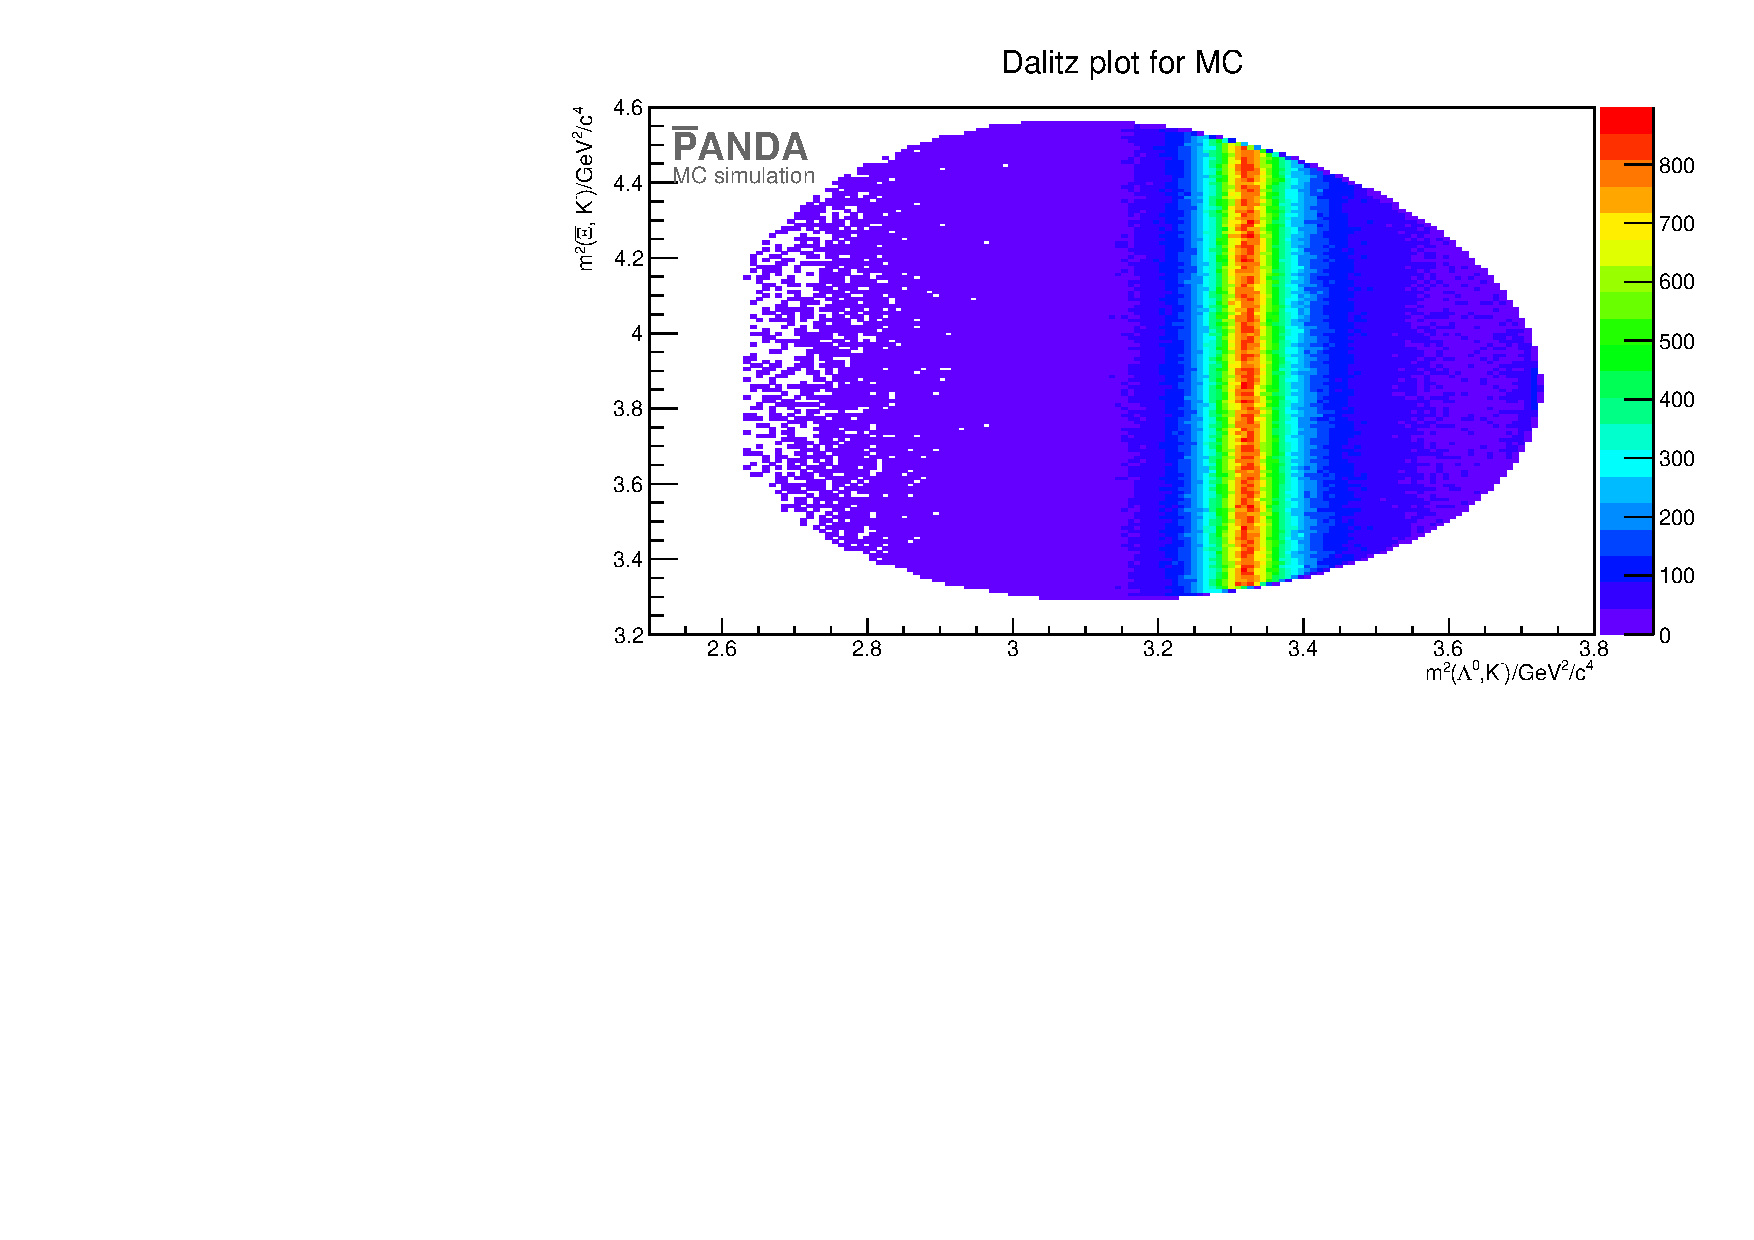
\includegraphics[width=0.6\textwidth]{./plots/Dalitzplot_MC.pdf}
	\caption{Dalitz plot for simulation. On x axis is the mass square of \lam  and \kminus and on the y axis there is the mass square of \anticascade and \kminus}
	\label{fig:eventgeneration_dalitz}
\end{figure}

